In this chapter, the background of data clumps will be discussed. A formal definition of data clumps will be presented (\ref{sec:data_clump_def}). ChatGPT will be discussed in section \ref{sec:chatgpt}. Also, the data clump type context format will be discussed. 

\section{Data clumps}\label{sec:data_clump_def}
The term \enquote{Data Clump} was coined by Martin Fowler as one possible code smell that can occur in source code. He describes data clumps as follows:

\begin{displayquote}
Data items tend to be like children: They enjoy hanging around together around in groups. Often you will see
the same three or four data items together in lots of
places: fields in a couple of classes, parameters in many
method signatures. \cite{fowler2019refactoring} 
\end{displayquote}

This definition is somewhat imprecise. It is not specified whether three or four data items are necessary. Also, \enquote{a couple of classes} and \enquote{in many method signatures} do not define concrete numbers. The author suggests checking whether the removal of one data clump item would have a significant effect on the coherence of the code.

A more precise and algorithmic definition of \enquote{data clumps} is provided by \cite{zhangImprovingPrecisionFowler2008}. They say a data clump  can be defined on the field or method-parameter levels. 
To be a method parameter data clump, a group of at least three variables must appear in multiple methods. Those variables must be duplicated, meaning they share the same name and data type. However, the inner order of the group does not need to be the same. 

These conditions often need to be more relaxed. For instance, methods can be inherited and overridden so that a group of parameters may appear in each derived class, thereby fulfilling the definition of a method parameter data clump. Since (except for the identifiers of the parameters) an overriding method must be the same as the overridden method, they are not considered data clumps.

For field data clumps, similar conditions apply. There must be at least three fields that appear in more than one class, and the names and data types of the variables must be the same, while the inner order may be different. Since in most programming languages, a field can have an additional access modifier (e.g., \textit{private}, \textit{static} etc. ), the access modifier should also be included to determine whether two groups of variables are identical and hence a data clump.  

The definition might also need to be more relaxed for both method and field data clumps. Two variables that have the same name but a compatible type in at least one direction  (e.g., \textit{int} and  \textit{double}), would be disregarded as a data clump according to the formalized definition. However, some would regard them as a data clump.

Also, modification of a variable's identifier might not change its meaning. For instance, typos can happen, or synonyms can be used so that an automatic algorithm might not discover the connection between two variables but requires knowledge of the semantics of the source code. \cite{zhangImprovingPrecisionFowler2008}


To conclude, the core definition of a data clump is clear. However, this definition still leaves out some edge cases that require a semantic understanding of the source code. 

An example of a data clump is shown in listing \ref{lst:math_stuff_java}
\begin{figure} [htbp!]
			\lstinputlisting
			[caption={Some operations on vectors},
			label={lst:math_stuff_java},
			captionpos=b,language=java, basicstyle=\footnotesize, tabsize=2, showstringspaces=false,  numbers=left]
			{figures/chapter2/dataClump/MathStuff.java}
		\end{figure}



Listing \ref{lst:math_stuff_java} contains three methods that execute some vector operations (calculation of length, sum of coordinates, and the maximum coordinate). 


It can be seen that  the snippet contains a method parameter data clump since the variables \textit{x}, \textit{y}, and  \textit{z} occur thrice.  These variables might be called \textbf{data clump items}
  
\subsection{Refactoring data clumps}
Fowler suggests two  steps to refactor a data clump:

In the  \textbf{Extract-Class}-step, a class with fields for each data clump item is extracted. A class for this purpose might already exist so that it can be re-used.

In the second step, \textbf{Preserve Whole Object} or \textbf{Introduce Parameter Object} might be applied. This means that the signature of the method is changed so that the extracted class replaces the data clump items, and all references to the method are changed accordingly.


To illustrate the suggested data clump refactoring process, listing \ref{lst:math_user_java} shows how the methods in \ref{lst:math_stuff_java} can be used. 


  \begin{figure} [htbp!]
			\lstinputlisting
			[caption={Some operations on vectors},
			label={lst:math_user_java},
			captionpos=b,language=java, basicstyle=\footnotesize, tabsize=2, showstringspaces=false,  numbers=left]
			{figures/chapter2/dataClump/MathUser.java}
	\end{figure}

In the first step, a new class can be extracted, which contains all data clump items as fields. It should also contain setters and getters to access the fields in an encapsulated manner. The class should be named so that its purpose is clear. Listing \ref{lst:coordinate_java} shows how such a class may look like. 

  \begin{figure} [htbp!]
			\lstinputlisting
			[caption={ Resulting Coordinate class},
			label={lst:coordinate_java},
			captionpos=b,language=java, basicstyle=\footnotesize, tabsize=2, showstringspaces=false,  numbers=left]
			{figures/chapter2/dataClump/Coordinate.java}
		\end{figure}

In the second step, a parameter object is introduced that replaces the three previous data clump items in each of the three methods of the \textit{MathStuff} class so that the signature only contains one parameter of type \textit{Coordinate}. Also, the calls in \textit{MathUsage} are refactored to reflect that change ( listing \ref{lst:math_stuff_refactored_java} and \ref{lst:math_user_refactored_java}). 

  \begin{figure} [htbp!]
			\lstinputlisting
			[caption={ Resulting Coordinate class},
			label={lst:math_stuff_refactored_java},
			captionpos=b,language=java, basicstyle=\footnotesize, tabsize=2, showstringspaces=false,  numbers=left]
			{figures/chapter2/dataClump/MathStuffRefactored.java}
		\end{figure}
  \begin{figure} [htbp!]
			\lstinputlisting
			[caption={ Resulting Coordinate class},
			label={lst:math_user_refactored_java},
			captionpos=b,language=java, basicstyle=\footnotesize, tabsize=2, showstringspaces=false,  numbers=left]
			{figures/chapter2/dataClump/MathStuffRefactored.java}
		\end{figure}

\section{ Data clumps Type Context }\label{sec:data_clump_format}

The \textbf{Data clumps Type Context} \cite{dataclump_type_context} is developed by Baumgartner et al. to establish a standard for reporting data clumps.

The format consists of three layers. In the outer layer, general project information is defined—for instance, the programming language or the location of the project.

In an inner layer, each detected data clump is described as a link between multiple method parameters or fields and another method parameters or fields. 

In the inner layer, each data clump item is linked to another data clump item, and information like the data type and identifier are described. 

\section{ChatGPT}\label{sec:chatgpt}

ChatGPT \cite{ChatGPT_url} is a \ac{LLM} developed by OpenAI and released in November 2022. As a \ac{LLM}, ChatGPT can interpret user queries and return an appropriate response. 

A query can be a question or a prompt directing ChatGPT to answer a question or provide some output. The range of topics ChatGPT can help with is basically unlimited. For instance, ChatGPT can help with math, history, politics, or coding topics. ChatGPT can also understand programming language and therefore, help developers to code. Since September 2023, ChatGPT can also process images \cite{ChatGPT_image}. However, it must be noted that ChatGPT may not always provide accurate responses since it is, in the end, just a language model without knowledge about the inherent meanings of its responses. 

The usage of ChatGPT is nevertheless somewhat restricted. For instance, content regarded as hate speech or used for illegal purposes will be suppressed.

Another essential feature of ChatGPT is the ability to store conversations. A conversation is a collection of queries and linked responses sent to ChatGPT. Using conversations, a user can refer to a previous query or response in a later query. For instance, if ChatGPT makes a mistake or misinterprets a query, a user can send another request connected to the previous request and point out the mistake or give more context, helping ChatGPT auto-correct itself. 

\subsection{Challenges on using Large Language Models}\label{sec:llm_challenges}

While LLM bring many advantages  and possibilities, using \ac{LLM}  successfully can be challenging. 

First of all \ac{LLM} are not trustworthy. They are often confident in their answers which nevertheless are wrong. This confidence can often be broken by asking subsequent questions which lead the \ac{LLM} to rethink the answer. however, doing this in an automatic way is challenging.

Additionally, \ac{LLM} use randomness in their answers which means that the same query can result in different replies. The factors influencing the reply are generally not known and should not be assumed. As a result, requirements regarding a specific output format, may be ignored by the model so that developers using a \ac{LLM} must always consider how to parse non-adhering output. 

Furthermore, \ac{LLM}s are usually black boxes. They do not give hindsight on how they came to a specific reply. While they can explain their reasoning, it is not possible to check the exact thought process.
While a query can consists of multiple parts, conditions, or requirements, a \ac{LLM} will not always adhere to all of these. It may weight some requirements, ignore other or interpret them wrongly so that the result is unexpected. A \ac{LLM} may also come to an intermediate result that it will not show at the end even though the intermediate result was correct or requested. Also no sources of the information is provided. 

Moreover, \ac{LLM}s do not have access to the latest information about a topic. They cannot access external sources like current news  and up-to-date documentation. Instead they employ a so-called cut-ff date. Only information before that cut-off date will be used. As of the time of writing this section, the cut-off date for ChatGPt is April  2023. However, the release was several months later.  

There also security issues with using  \ac{LLM} like ChatGPT. If a model is asked to generate or refactor code, one cannot trust that the code is safe to use. As a result of the cut-off date, the code might use operations that are considered deprecated or even unsafe to use because security vulnerabilities have been detected in the meantime. As a result, the developer needs to verify whether the code is safe to use which is another burden. 

Furthermore, it is not out of the question that a malicious attacker might change the query or the reply of a \ac{LLM}. Therefore, using such a model might be a feasible way to hack systems or create damage which is difficult to detect and prevent. 

\section{Related Research}
The problem of data clump detection and refactoring is addressed in multiple papers. Also the  use of large language models in software development is a fairly recent rearch topic. In this section, research to both topics will be outlined: 

\subsection{Related to data clumps}
Baumgartner et al.  developed a live code smell detection plugin for IntelliJ that can detect, report, and refactor data clumps without significantly impacting performance. However, the tool is semi-automatic, meaning the developer must still actively approve the data clump refactoring and suggest a suitable class name for the extracted class. \cite{BaumgartnerAP23}

As outlined in section \ref{sec:data_clump_def}, the definition of data clump by Fowler \cite{fowler2019refactoring} is somewhat ambiguous because no clear criteria to determine data clumps is established. Zang et al. \cite{zhangImprovingPrecisionFowler2008} creates a more algorithmic approach to determine whether a data clump exists. This approach is also explained in section \ref{sec:data_clump_def}. The authors also provide more precise definitions of other code smells like \enquote{message chains} or \enquote{speculative generality}. By interviewing four software development experts about the code smell definitions the authors developed, they find that their new data clump definition receives relatively more disagreement than other definitions, which the authors explain are the results of not covering edge cases in the definitions. 


Hall et al. analyzed the impact of code smells (including data clump) on the occurrence of faults in three open-source software projects. They find that data clumps have a mixed correlation to faults because, in two of the three projects analyzed, the correlation of data clumps per \ac{LOC} to detected faults is negative for two projects and positive for one project. This rejects their hypothesis that data clumps do not affect faults, and the authors suggest that the application domain and the development context need to be considered before the time-consuming refactoring of data clumps since their impact is not predictable.  \cite{hallCodeSmellsHave2014}

\subsection{Related to large language models in software development}

White et al. \cite{White2023ChatGPTPP} outline how ChatGPT can be used in software development to improve the worklflow of developers. This includes  exploration of requirements, removing ambiguity in technical specification, or describing source code. The authos suggest specific prompts to elicit a suitable response from ChatGPt.

In case of refactoring, the author suggest that ChatGPT is able to refactor code with multiple prompts. For instance, ChatGPT can refactor based on a well known design pattern name, multiple examples on how to refactor the code, or a more lengthy requirements description. The exact success of each prompt is however dependent on how ChatGPT is trained and should be scrutinized manually. 

Cao et al. \cite{cao2023study} focus on using ChatGPT for fixing deep learning programs. Those are programs that cannot be understood only by their source code alone, but are are largely influenced by underlying data like  neural networks etc. This makes finding faults more difficult. The study finds out that ChatGPT can find code smells and detect faults. Without giving instructions however, ChatGPT will tend to return code smells and outdated API calls while not finding other bugs. 



\section{Language Server Protocol}
The \ac{LSP}  \cite{lsp_website} is a protocol developed by Microsoft to create a language-independent interface for code-related operations. 
The \ac{LSP}  describes a server and a client who communicate to each other using the JSON-Remote-Remote-Process-Call protocol \cite{json_rpc}. 

In general, the client can be anything that works with source code but has no detailed knowledge of a specific programming language. For instance, an \ac{IDE}, an editor or a refactoring tool can be described as a client.

The client starts a server based on a programming language. The server has a inherent knowledge of one ore more programming languages and can provide source-code-related functionality. For instance, the server can rename a variable, find the usages of a method, or inform the client about compiler errors. 

Initially, client and server some information to set-up. This includes the path to the project that the server should load and information about what functionality each of them support. These functionalities are named \textit{Capabilities}. For example, the server can announce that it supports renaming variables while the client show error messages. Hence, server and client can interact in a manner such that no unsupported messages are transferred.

Figure \ref{fig:lsp_usage} illustrates how the \ac{LSP} works in practice after the initialization process. 
\begin{figure}
    \centering
    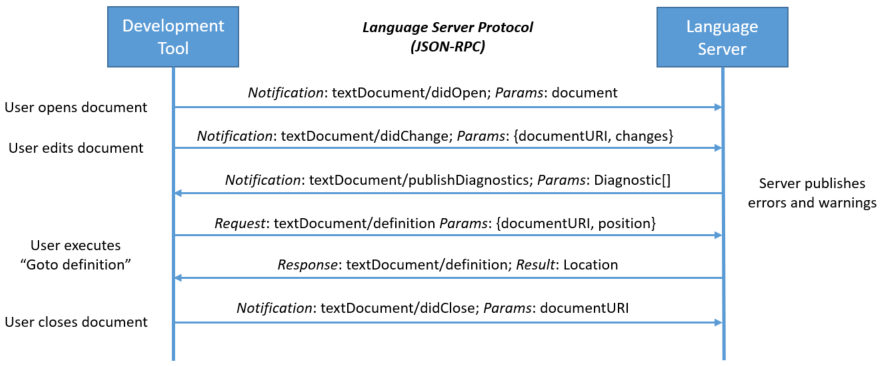
\includegraphics{figures/chapter2/language-server-sequence.png}
    \caption{Example usage of the Language Server Protocol}
    \label{fig:lsp_usage}
    \cite{lsp_website}
\end{figure}

After the server has successfully started by the client, a user can open a document (e.g. source code file). The request to open the document is submitted to the server. From now one, the server may not rely on the file system since that might be not the current version of the opened document. 

The client can now inform the server about some changes (e.g. adding a new method). The server can in the meantime inform the client about syntactical errors which the client might show to the user of the client.

Afterwards, the client requests the definition of a method or variable, and the server returns a response with the requested data.

In the end, the client can save the document and notify the server that the document was closed which means that the physical file of the document represents the current version of the document again. 